\chapter{Sistema actual: plataforma FAdA y el bucle de control MAPE-K \foreign{english}{Lite}}
\label{chap:sistema_original}

\begin{wrapfigure}{r}{0.3\linewidth}
  \vspace{5pt}
  \centering
  
\includegraphics[scale=0.45]{cap_sistema_original/images/fada-logo}
  \vspace{2pt}
\end{wrapfigure}

La plataforma FAdA\footnote{Página oficial: \url{http://fada.tatami.webs.upv.es/}} está enfocada en el desarrollo de sistemas autoadaptativos. Es un desarrollo del grupo PROS/Tatami\footnote{Página oficial: \url{http://www.pros.webs.upv.es/}} del instituto VRAIN/UPV\footnote{Página oficial: \url{https://vrain.upv.es/}}. Está compuesta por una serie de herramientas y guías metodológicas. Entre ellas encontramos extensiones de modelado para el IDE Eclipse, generadores de código y diversas implementaciones de bucles de control genéricos. Uno de estos bucles es aquel que queremos adaptar a entornos \foreign{english}{cloud}: el bucle MAPE-K \foreign{english}{Lite}.

En este capítulo haremos una breve introducción a la plataforma y las herramientas que la componen. Introduciremos conceptos como los servicios \foreign{english}{adaptive ready} y describiremos el funcionamiento del bucle MAPE-K \foreign{english}{Lite}.

\section{Desarrollo de servicios \foreign{english}{Adaptive Ready}}

Comenzaremos describiendo la extensión para el IDE Eclipse. Tomando una aproximación de \textbf{desarrollo dirigido por modelos} (o \foreign{english}{model driven development}, MDD), esta herramienta permite diseñar soluciones autoadaptativas. Las soluciones están compuestas por especificaciones de servicios \textbf{\foreign{english}{adaptive ready}} (ARS). \cite{fonsServiciosAdaptivereadyPara2021}

Los servicios \foreign{english}{adaptive ready} implementan la funcionalidad y delegan en un bucle de control externo la responsabilidad de gestionar las adaptaciones. Para ello ofrecen una serie de interfaces, las sondas y efectores, que permiten recibir comandos desde el bucle. En la figura \ref{fig:adaptive-ready-services} se muestra un esquema del servicio y de cómo el bucle orquesta la solución.

La plataforma ofrece una serie de generadores de código. A partir de los modelos es posible generar todo el código de infraestructura de las interfaces de adaptación. Para integrarlas en los servicios, el desarrollador deberá importarlas e implementar la lógica asociada a los comandos. Dependiendo del tipo de despliegue por el que optemos, pueden generarse para microservicios, módulos OSGi\footnote{Página oficial: \url{https://www.osgi.org}.}, entre otros.

\pagebreak

Para operar estas soluciones, la plataforma ofrece distintas implementaciones de bucles de control. Cuál emplear dependerá del modelo de despliegue de la aplicación. Disponemos de soluciones para gestionar microservicios sobre la plataforma Kubernetes\cite{fonsServiciosAdaptivereadyPara2021}, otros que permiten operar componentes OSGi\footnote{Página oficial: \url{https://www.osgi.org}.}, etc. En este trabajo nos centraremos en una versión reducida del bucle de control para microservicios: MAPE-K \foreign{english}{Lite}.

\begin{figure}[htb]
  \centering
  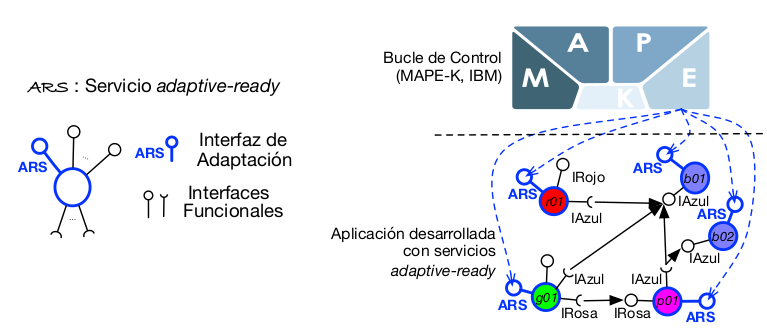
\includegraphics[scale=0.4]{cap_sistema_original/images/adaptive-ready-services}
  \caption[Servicio adaptive-ready y Bucle MAPE-K sobre arquitectura de mi-
  croservicios adaptive-ready.]{Servicio adaptive-ready (izquierda) y Bucle MAPE-K sobre arquitectura de microservicios adaptive-ready (derecha). Obtenida de \cite{fonsServiciosAdaptivereadyPara2021}.}
  \label{fig:adaptive-ready-services}
\end{figure}


\section{Bucle de control MAPE-K \foreign{english}{Lite}}

El bucle de control MAPE-K \foreign{english}{Lite} de FAdA nos permite gestionar soluciones autoadaptativas basadas en microservicios. Es una versión reducida del bucle presentado en \cite{fonsServiciosAdaptivereadyPara2021}. Sigue la arquitectura MAPE-K descrita en la sección \ref{sec:bucles-mapek}. En su implementación actual, se despliega como un servicio monolítico al nivel de la solución autoadaptativa. Todos sus componentes, tanto del bucle como los del recurso manejado (monitores, reglas...), se ejecutan dentro del mismo proceso.

El bucle de control es genérico. No está acoplado a un dominio o solución concreta. Además, pueden hacer uso de él varios sistemas a la vez. El proceso acepta como entradas las mediciones de las sondas y emite comandos dirigidos a los efectores del recurso manejado. En nuestro caso, los \foreign{english}{touchpoints} de los servicios \foreign{english}{adaptive ready}. En la figura \ref{fig:bucle-mapek3} mostramos un modelo que detalla el flujo de control e información dentro de sus etapas.

\begin{figure}[htb]
  \centering
  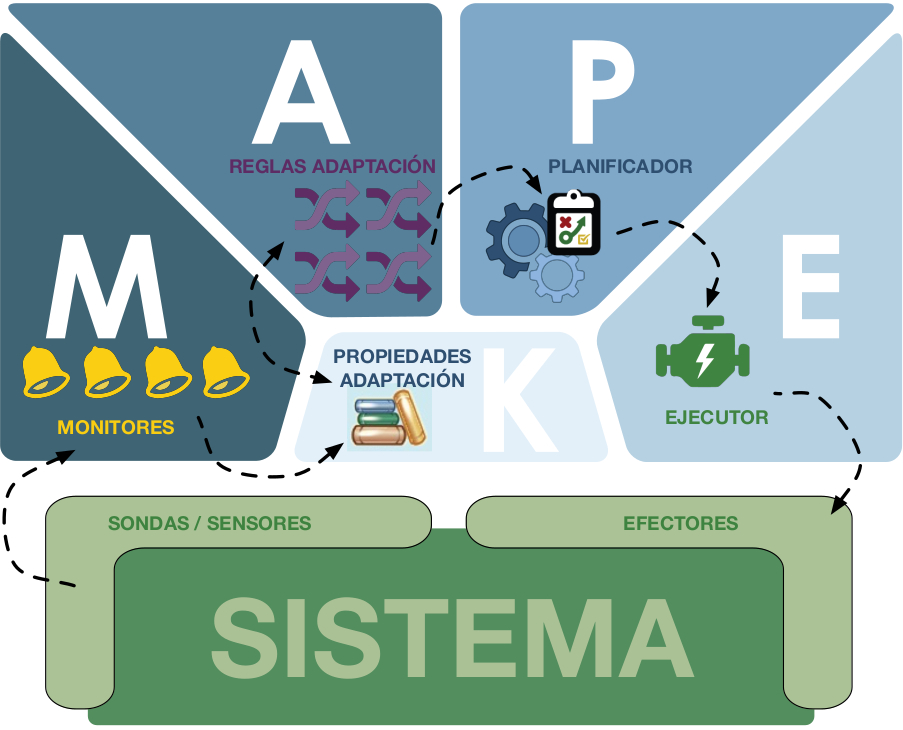
\includegraphics[scale=1]{cap_introduccion/images/bucle-mape-k}
  \caption[Arquitectura del bucle MAPE-K \foreign{english}{lite}. El flujo de información y de control entre las etapas del bucle están representados con flechas.]{Arquitectura del bucle MAPE-K \foreign{english}{lite}. El flujo de información y de control entre las etapas del bucle están representados con flechas. Obtenida de \cite{fonsEspecificacionSistemasAutoadaptativos2021}}
  \label{fig:bucle-mapek3}
\end{figure}

\subsection{Estructura del bucle}

En la sección \ref{sec:estructura-mape-k} ya describimos la estructura de un bucle MAPE-K típico. Como se puede ver en la figura \ref{fig:bucle-mapek3}, este no difiere mucho en su implementación. Sigue la misma secuencia de monitorización, análisis, planificación y ejecución. Para implementarlas cuenta también con los mismos componentes: sondas, monitores, módulo de análisis, planificador, ejecutor y efectores. Pero sí que hay una faceta en la que queremos hacer hincapié: el uso de reglas de adaptación en la etapa de análisis.

\subsubsection{Módulo de análisis y reglas de adaptación}

El módulo de análisis del bucle de control se ha implementado mediante un conjunto de \textbf{reglas de adaptación}. Se trata de la codificación de heurísticas que nos permiten corregir u optimizar el funcionamiento del sistema. En base a los reportes de los monitores, se buscan oportunidades para mejorar la configuración en tiempo de ejecución.

Las reglas pueden ser generales o especificas a un recurso manejado concreto. Se dividen en dos componentes: la condición y la propuesta de cambio. La \textbf{condición} es una función que determina si es necesario ejecutar la acción. Se define a partir de las propiedades de adaptación del conocimiento. Esta se evaluará en tiempo de ejecución cuando se produzca un cambio en la configuración o se obtenga nueva información del entorno.

Por otro lado, la \textbf{propuesta de cambio} describe cuál debería ser la siguiente configuración del sistema: qué componentes deben estar o no presentes, qué conexiones entre ellos deben existir y sus parámetros de configuración. Las reglas enviarán esta propuesta al planificador. El planificador analizará el estado actual y pautará qué \textbf{acciones} son necesarias para alcanzar el estado deseado. Sobre los componentes y conexiones que no se especifique nada se mantendrán como estaban.

\subsubsection{Operadores arquitectónicos}

Las acciones se especifican usando \textbf{operadores arquitectónicos}. \cite{garlanIncreasingSystemDependability2003} Dependiendo del estilo arquitectónico del recurso manejado, tendremos disponibles unos operadores determinados. El bucle de control que nos ocupa es específico para gestionar soluciones basadas en microservicios. Por tanto, ofrecerá los operadores correspondientes a este estilo. En \cite{fonsEspecificacionSistemasAutoadaptativos2021} podemos encontrar los cinco tipos que ofrece:

\begin{itemize}
  \item \textbf{Desplegar servicios} (\textbf{\foreign{english}{deploy}}): Añadimos una nueva instancia de un servicio.

  \item \textbf{Eliminar servicios} (\textbf{\foreign{english}{undeploy}}): Eliminamos una instancia de un servicio.

  \item \textbf{Enlazar servicios} (\textbf{\foreign{english}{bind}}): Añadimos una conexión entre dos servicios. A partir de entonces podrán comunicarse.

  \item \textbf{Desenlazar servicios} (\textbf{\foreign{english}{unbind}}): Eliminamos una conexión existente entre dos servicios. Ya no podrán comunicarse.

  \item \textbf{Cambiar configuración} (\textbf{\foreign{english}{set parameter}}): Modificamos un parámetro de configuración de un servicio.
\end{itemize}

En la figura \ref{fig:adaptaciones-microservicios} mostramos un ejemplo de los efectos de estas acciones en la arquitectura del sistema.

\begin{figure}[htb]
  \centering
  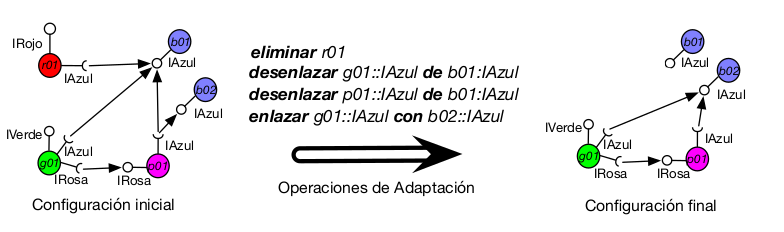
\includegraphics[scale=1.8]{cap_sistema_original/images/adaptaciones}
  \caption[Ejemplo de adaptaciones en un sistema basado en microservicios.]{Ejemplo de adaptaciones en un sistema basado en microservicios. Imagen original obtenida de \cite{fonsServiciosAdaptivereadyPara2021}}
  \label{fig:adaptaciones-microservicios}
\end{figure}

\subsubsection{Ejemplo de regla de adaptación}

Para presentar una regla de adaptación, nos adelantaremos un poco y tomaremos de ejemplo una de las definidas en el caso de estudio (capítulo \ref{chap:caso_estudio}). Esta regla pertenece a un sistema de climatización encargado de regular la temperatura de una habitación. Este cuenta con un termómetro (la sonda) y un sistema de aire acondicionado (el recurso manejado). Además, el recurso cuenta con una serie de efectores que permiten cambiar el modo de funcionamiento: enfriar, calentar o apagado.

Esta regla en concreto se encarga de activar el modo refrigeración. Para ello, en su condición comprueba que la temperatura supere un umbral definido por el usuario; y que no esté enfriando ya la estancia. De cumplirse, se especifica que en la siguiente configuración del sistema deberá estar presente el componente de aire acondicionado. Este debe deberá tener activo el modo de enfriamiento.

Para especificar las reglas usaremos la notación SAS. \cite{fonsEspecificacionSistemasAutoadaptativos2021} Esta define una serie de pautas para describir su condición y representar la configuración que solicitará el cuerpo de la regla. En la tabla \ref{tab:adaption-rules-example} presentamos la especificación de esta regla.

\begin{longtable}{|r p{12.8cm}|}
    \hline
    \textbf{Regla:} & \texttt{EnableAirConditionerCoolingModeWhenTemperatureThresholdExceeded}  \\
    \textbf{Descripción:} & Activa el aire acondicionado en modo enfriar cuando la temperatura sea superior al umbral de calor.  \\
    \textbf{Condición:} & \emph{airconditioner-mode} != \emph{Cooling} \textbf{AND} \emph{temperature} >= \emph{hot-temperature-threshold}  \\
    \textbf{Cuerpo:} &  \\
    & 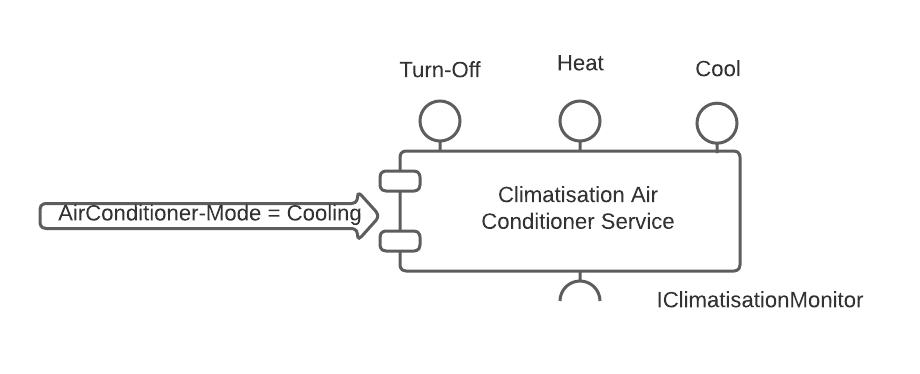
\includegraphics[scale=0.75]{cap_caso-estudio/images/adaption-loop-rule-cooling} \\
    \hline

  \caption{Ejemplo de especificación de regla de adaptación con la notación SAS.}
  \label{tab:adaption-rules-example}
\end{longtable}

El planificador del sistema recibirá esta propuesta de cambio y tendrá que determinar qué acciones son necesarias para alcanzarlo. Por ejemplo, si el componente del aire acondicionado estuviera activo, sólo se pautaría la acción para cambiar el parámetro \texttt{Mode} para que tenga el valor \texttt{Cooling}.
